\section{Evaluación, comparación de modelos y resultados}
\label{sec:evaluacion}

%
% Para citar: 
% 	(ver Sección~\ref{sec:dataset_arquitectura})
% 	como se describe en la Sección~\nameref{sec:dataset_arquitectura})
%

\subsection{Resultados experimentales}
\label{sec:resultados_exp}

\begin{comment}
	- Presentación de los resultados finales:
	- Tablas y/o gráficos para las métricas más relevantes (MAE, RMSE, R2, MAPE...) para cada experimento y cada mejor modelo.
	- Comparativa directa entre MLP y Trafficformer para cada source.
	- Visualizaciones clave (si tienes heatmaps, gráficas de error, etc.).
\end{comment}

Para cada una de las tres fuentes de datos disponibles (\texttt{sourceId} = 1, 2 y 5), se ha seleccionado el mejor modelo entrenado para cada una de las dos arquitecturas evaluadas: \texttt{MLP} y \texttt{Trafficformer}. La selección se ha realizado tomando como criterio el valor mínimo de la métrica de pérdida sobre el conjunto de validación (\texttt{val\_loss}) entre todas las combinaciones de hiperparámetros evaluadas durante el proceso experimental.

En el \hyperref[anexo:resultados_exp]{Anexo~F} se puede consultar la tabla completa de todos los experimentos llevados a cabo junto con los resultados de todas las métricas obtenidas.

En la tabla~\ref{tab:mejores_modelos} se muestran los modelos seleccionados junto con sus respectivas métricas sobre el conjunto de test, así como los valores clave de los hiperparámetros empleados.

\begin{table}[H]
	\centering
	\small
	\caption{Resultados de los mejores modelos por combinación \texttt{sourceId}--arquitectura}
	\label{tab:mejores_modelos}
	\begin{tabularx}{\textwidth}{c | c | c | c | c | c | c | c }
		\toprule
		\textbf{SID} & \textbf{M} & \textbf{EP} & \textbf{VTL} & \textbf{VTMAE} & \textbf{VTRMSE} & \textbf{VTMAPE} & \textbf{VTR2} \\
		\midrule
		1 & mlp           & 67 & 0.000 & 25.327/25.466 & 50.904/38.489 & 1.826/1.853 & 0.743/0.759 \\
		1 & trafficformer & 30 & 0.143 & 19.300/19.125 & 44.298/30.784 & 1.718/1.745 & 0.797/0.822 \\
		2 & mlp           & 30 & 0.000 & 30.967/31.017 & 38.144/38.177 & 1.75e14/1.82e14 & 0.868/0.866 \\
		2 & trafficformer & 96 & 0.002 & 5.787/5.832 & 15.356/15.046 & 1.31e3/1.51e3 & 0.983/0.982 \\
		5 & mlp           & 39 & 0.000 & 216.265/213.850 & 345.766/343.603 & 4.85e5/4.83e5 & 0.523/-1.797 \\
		5 & trafficformer & 29 & 0.153 & 176.356/175.975 & 308.041/306.134 & 1.74e5/1.74e5 & 0.703/0.640 \\
		\bottomrule
	\end{tabularx}
	\vspace{0.5em}
	\begin{minipage}{0.98\textwidth}
	\footnotesize
	\textbf{Leyenda de columnas:} \\
	\textbf{SID}: sourceId. \\
	\textbf{M}: Modelo. \\
	\textbf{EP}: Epoch óptima. \\
	\textbf{VTL}: Validation \& Test Loss. \\
	\textbf{VTMAE}: Validation \& Test MAE. \\
	\textbf{VTRMSE}: Validation \& Test RMSE. \\
	\textbf{VTMAPE}: Validation \& Test MAPE. \\
	\textbf{VTR2}: Validation \& Test $R^2$. \\
	Los valores muy grandes se muestran en notación científica (\texttt{a.eb} significa $a \times 10^{b}$). Decimales reducidos para mejorar la presentación.
	\end{minipage}
\end{table}

%%

A continuación se muestran, para cada una de las combinaciones óptimas de fuente de datos (\texttt{sourceId}) y arquitectura (\texttt{MLP} y \texttt{Trafficformer}), las curvas de evolución de las principales métricas durante el entrenamiento. Estas gráficas permiten visualizar el comportamiento del proceso de aprendizaje en términos de error (loss), precisión (MAE, MAPE, MSE, RMSE), y capacidad explicativa ($R^2$), tanto en entrenamiento como en validación. De este modo, se facilita la identificación de fenómenos de sobreajuste, convergencia y diferencias entre arquitecturas y datasets.

Cada figura agrupa, en formato compacto, las seis métricas principales para cada modelo, mostrando la evolución época a época.

\begin{figure}[H]
	\centering
	\begin{minipage}{0.48\textwidth}
		\centering
		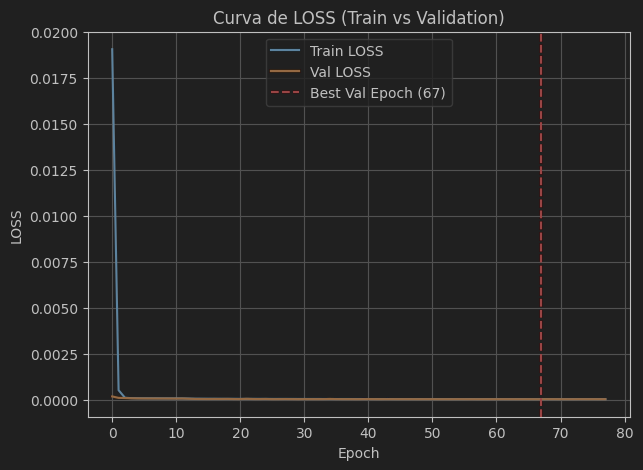
\includegraphics[width=\linewidth]{includes/cap5/graphs/sid1_mlp_loss.png}
		\subcaption{Loss}
		\vspace{0.2cm}
		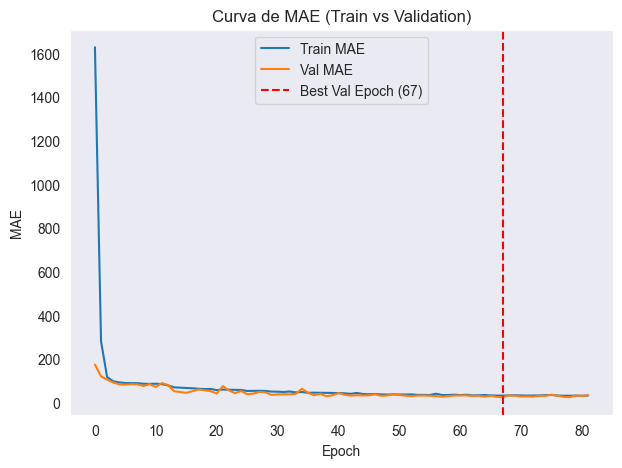
\includegraphics[width=\linewidth]{includes/cap5/graphs/sid1_mlp_mae.png}
		\subcaption{MAE}
		\vspace{0.2cm}
		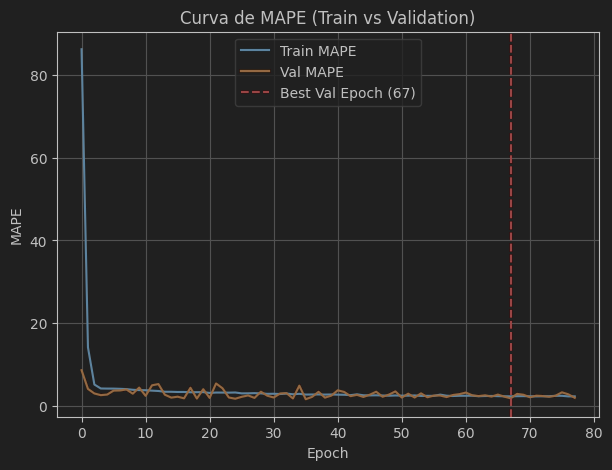
\includegraphics[width=\linewidth]{includes/cap5/graphs/sid1_mlp_mape.png}
		\subcaption{MAPE}
	\end{minipage}
	\hfill
	\begin{minipage}{0.48\textwidth}
		\centering
		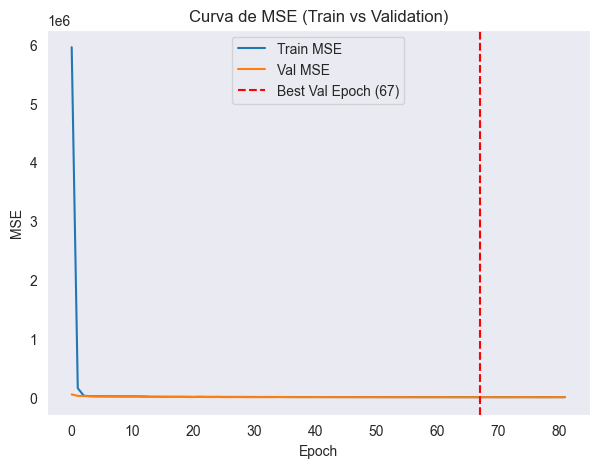
\includegraphics[width=\linewidth]{includes/cap5/graphs/sid1_mlp_mse.png}
		\subcaption{MSE}
		\vspace{0.2cm}
		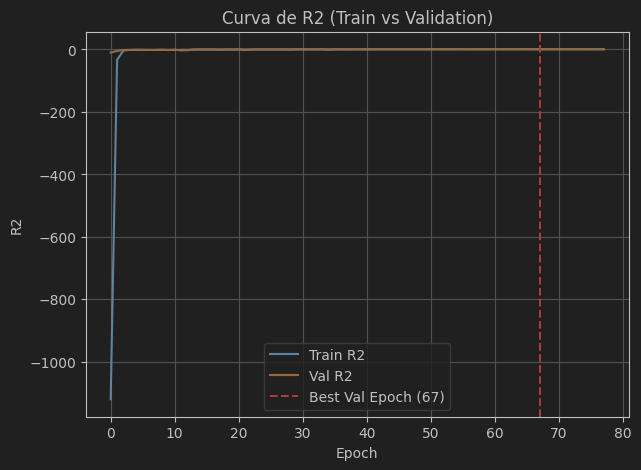
\includegraphics[width=\linewidth]{includes/cap5/graphs/sid1_mlp_r2.png}
		\subcaption{$R^2$}
		\vspace{0.2cm}
		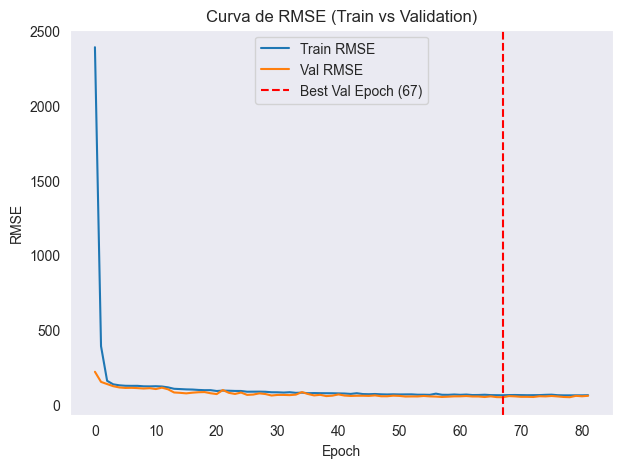
\includegraphics[width=\linewidth]{includes/cap5/graphs/sid1_mlp_rmse.png}
		\subcaption{RMSE}
	\end{minipage}
	\caption{Curvas de entrenamiento para el modelo \texttt{MLP} con sourceId 1.}
	\label{fig:curvas_sid1_mlp}
\end{figure}

\begin{figure}[H]
	\centering
	\begin{minipage}{0.48\textwidth}
		\centering
		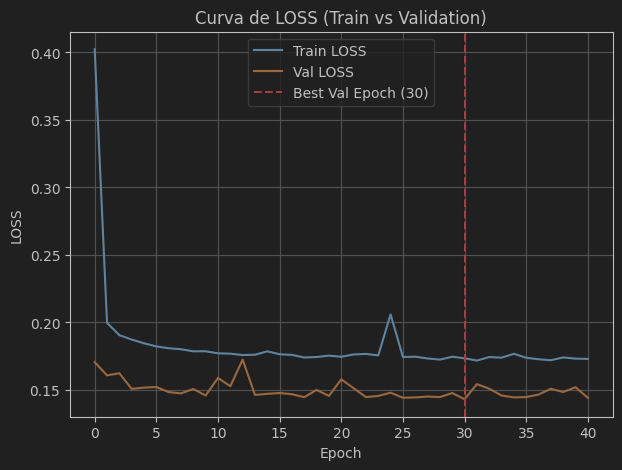
\includegraphics[width=\linewidth]{includes/cap5/graphs/sid1_trafficformer_loss.png}
		\subcaption{Loss}
		\vspace{0.2cm}
		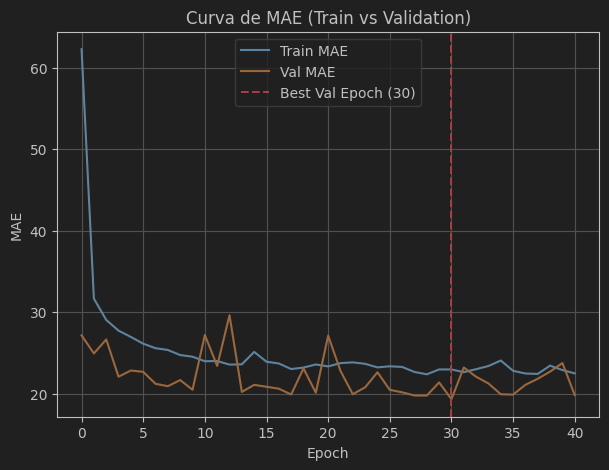
\includegraphics[width=\linewidth]{includes/cap5/graphs/sid1_trafficformer_mae.png}
		\subcaption{MAE}
		\vspace{0.2cm}
		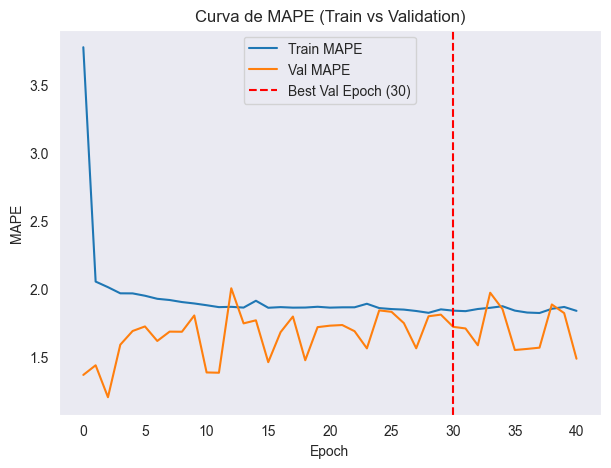
\includegraphics[width=\linewidth]{includes/cap5/graphs/sid1_trafficformer_mape.png}
		\subcaption{MAPE}
	\end{minipage}
	\hfill
	\begin{minipage}{0.48\textwidth}
		\centering
		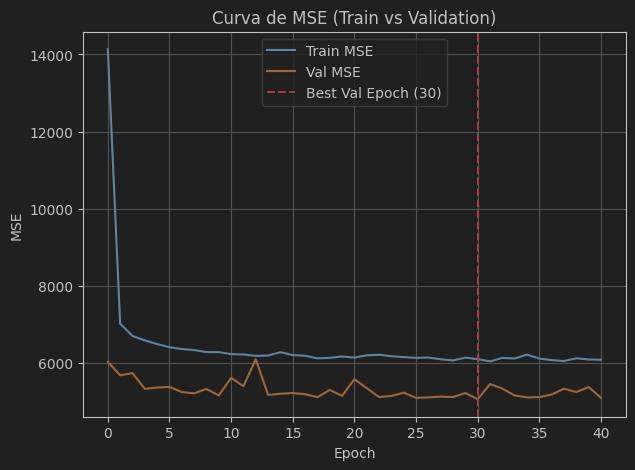
\includegraphics[width=\linewidth]{includes/cap5/graphs/sid1_trafficformer_mse.png}
		\subcaption{MSE}
		\vspace{0.2cm}
		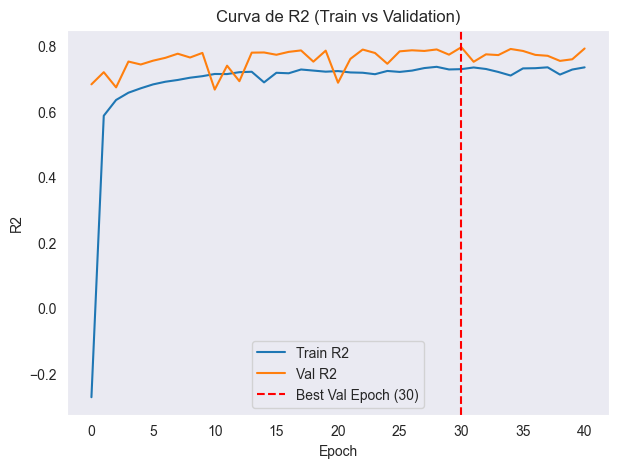
\includegraphics[width=\linewidth]{includes/cap5/graphs/sid1_trafficformer_r2.png}
		\subcaption{$R^2$}
		\vspace{0.2cm}
		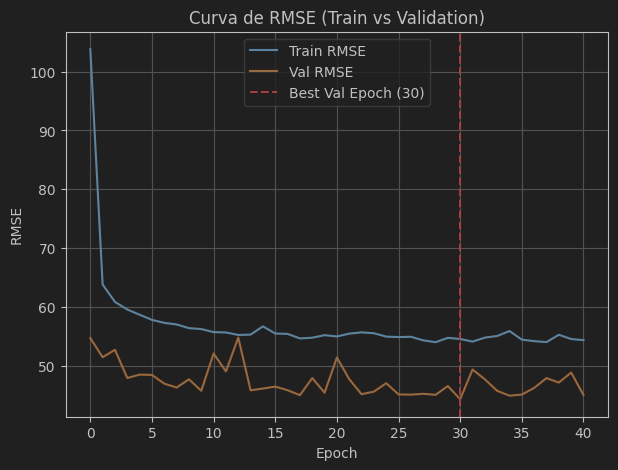
\includegraphics[width=\linewidth]{includes/cap5/graphs/sid1_trafficformer_rmse.png}
		\subcaption{RMSE}
	\end{minipage}
	\caption{Curvas de entrenamiento para el modelo \texttt{Trafficformer} con sourceId 1.}
	\label{fig:curvas_sid1_trafficformer}
\end{figure}

%%

\begin{figure}[H]
	\centering
	\begin{minipage}{0.48\textwidth}
		\centering
		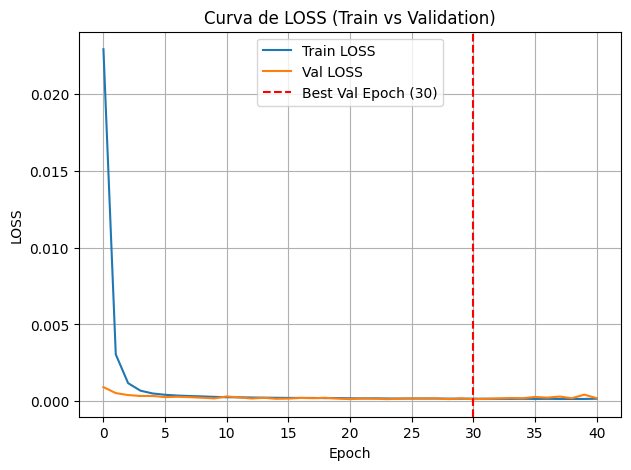
\includegraphics[width=\linewidth]{includes/cap5/graphs/sid2_mlp_loss.png}
		\subcaption{Loss}
		\vspace{0.2cm}
		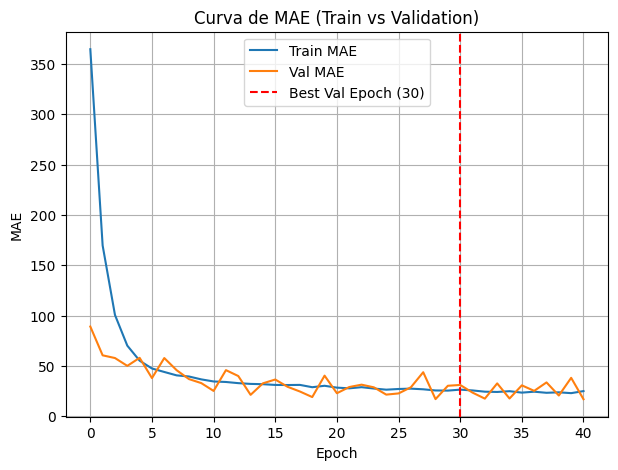
\includegraphics[width=\linewidth]{includes/cap5/graphs/sid2_mlp_mae.png}
		\subcaption{MAE}
		\vspace{0.2cm}
		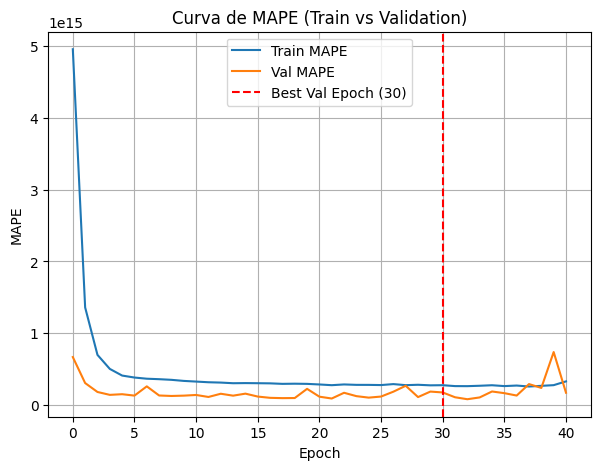
\includegraphics[width=\linewidth]{includes/cap5/graphs/sid2_mlp_mape.png}
		\subcaption{MAPE}
	\end{minipage}
	\hfill
	\begin{minipage}{0.48\textwidth}
		\centering
		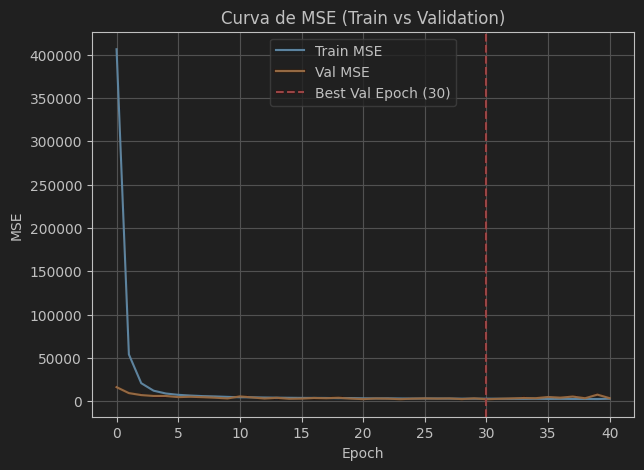
\includegraphics[width=\linewidth]{includes/cap5/graphs/sid2_mlp_mse.png}
		\subcaption{MSE}
		\vspace{0.2cm}
		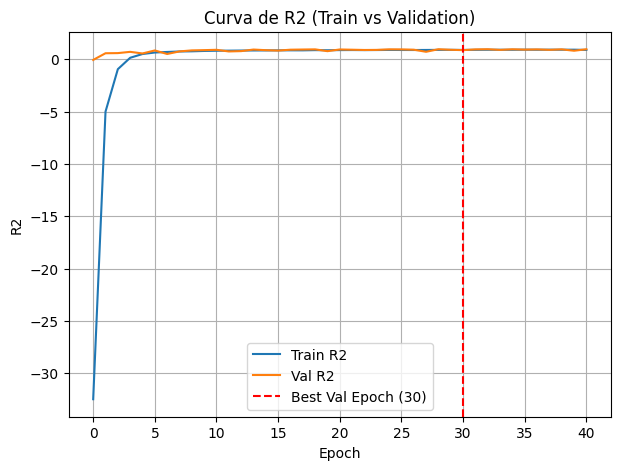
\includegraphics[width=\linewidth]{includes/cap5/graphs/sid2_mlp_r2.png}
		\subcaption{$R^2$}
		\vspace{0.2cm}
		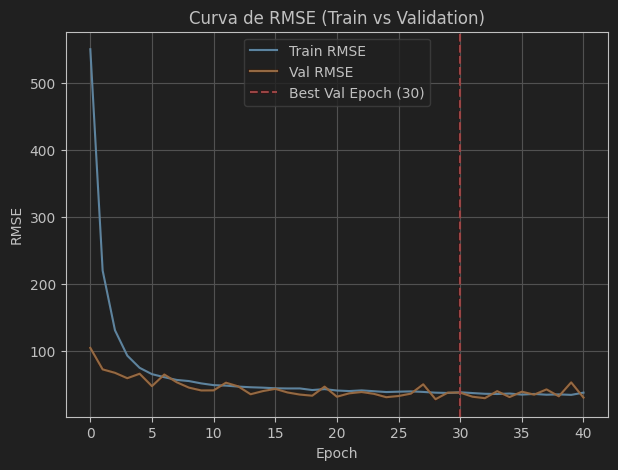
\includegraphics[width=\linewidth]{includes/cap5/graphs/sid2_mlp_rmse.png}
		\subcaption{RMSE}
	\end{minipage}
	\caption{Curvas de entrenamiento para el modelo \texttt{MLP} con sourceId 2.}
	\label{fig:curvas_sid2_mlp}
\end{figure}

\begin{figure}[H]
	\centering
	\begin{minipage}{0.48\textwidth}
		\centering
		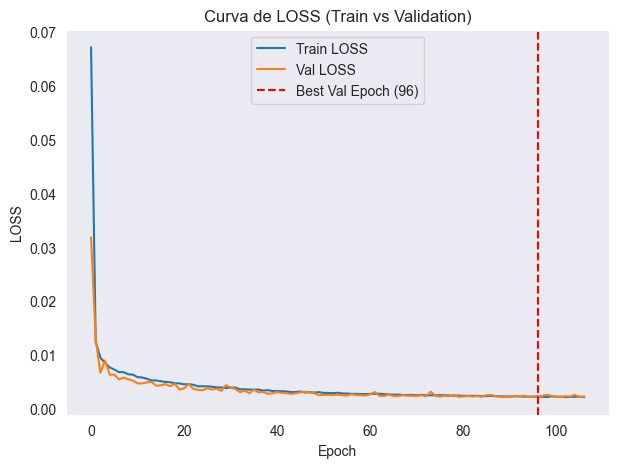
\includegraphics[width=\linewidth]{includes/cap5/graphs/sid2_trafficformer_loss.png}
		\subcaption{Loss}
		\vspace{0.2cm}
		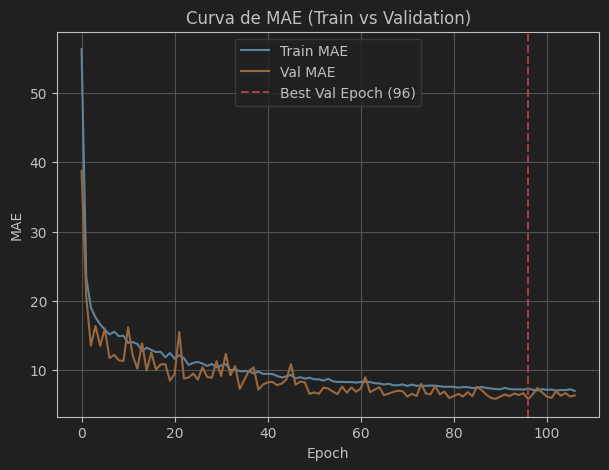
\includegraphics[width=\linewidth]{includes/cap5/graphs/sid2_trafficformer_mae.png}
		\subcaption{MAE}
		\vspace{0.2cm}
		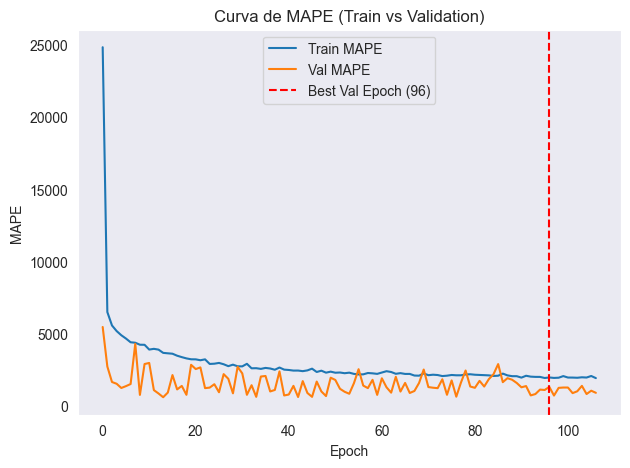
\includegraphics[width=\linewidth]{includes/cap5/graphs/sid2_trafficformer_mape.png}
		\subcaption{MAPE}
	\end{minipage}
	\hfill
	\begin{minipage}{0.48\textwidth}
		\centering
		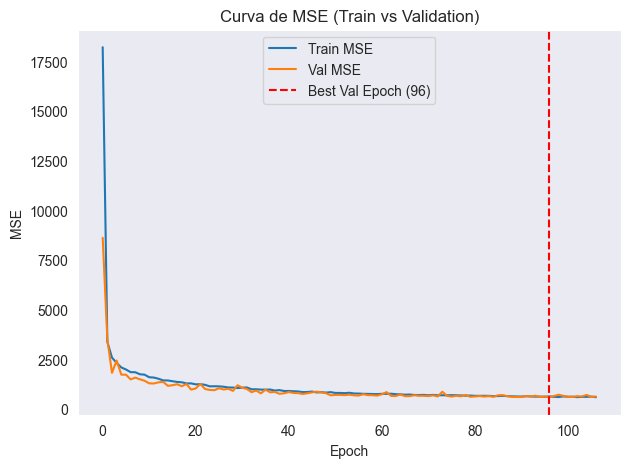
\includegraphics[width=\linewidth]{includes/cap5/graphs/sid2_trafficformer_mse.png}
		\subcaption{MSE}
		\vspace{0.2cm}
		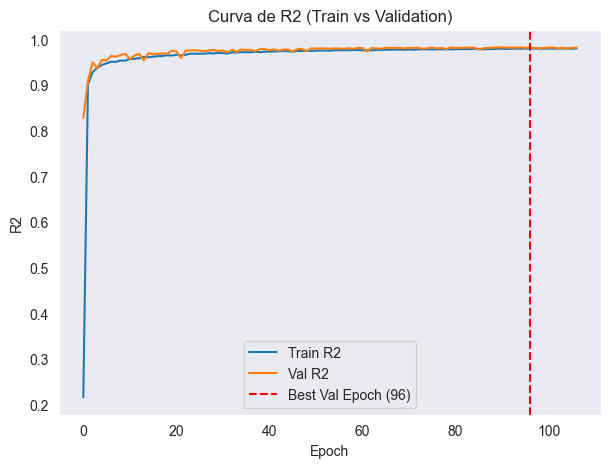
\includegraphics[width=\linewidth]{includes/cap5/graphs/sid2_trafficformer_r2.png}
		\subcaption{$R^2$}
		\vspace{0.2cm}
		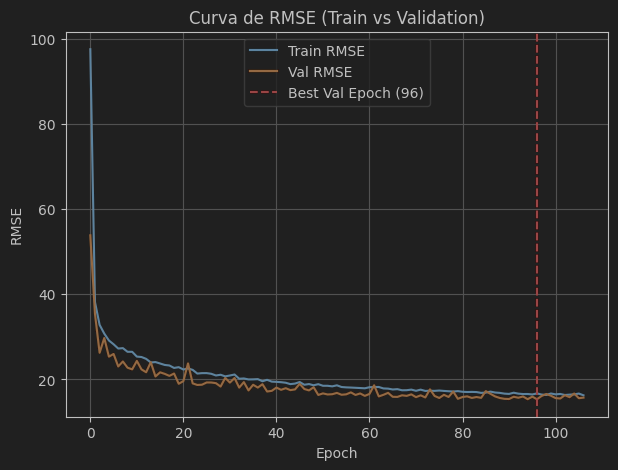
\includegraphics[width=\linewidth]{includes/cap5/graphs/sid2_trafficformer_rmse.png}
		\subcaption{RMSE}
	\end{minipage}
	\caption{Curvas de entrenamiento para el modelo \texttt{Trafficformer} con sourceId 2.}
	\label{fig:curvas_sid2_trafficformer}
\end{figure}

%%

\begin{figure}[H]
	\centering
	\begin{minipage}{0.48\textwidth}
		\centering
		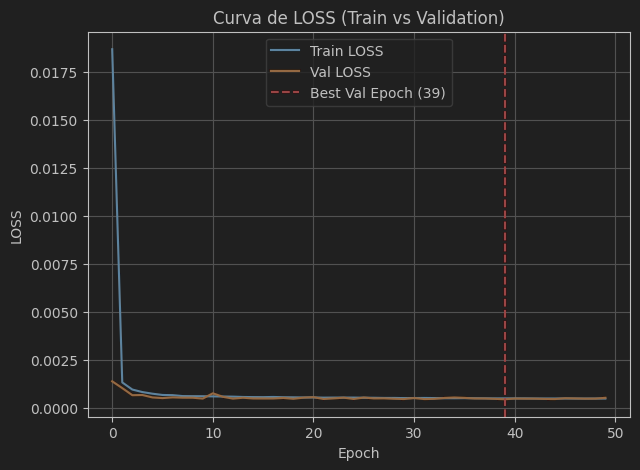
\includegraphics[width=\linewidth]{includes/cap5/graphs/sid5_mlp_loss.png}
		\subcaption{Loss}
		\vspace{0.2cm}
		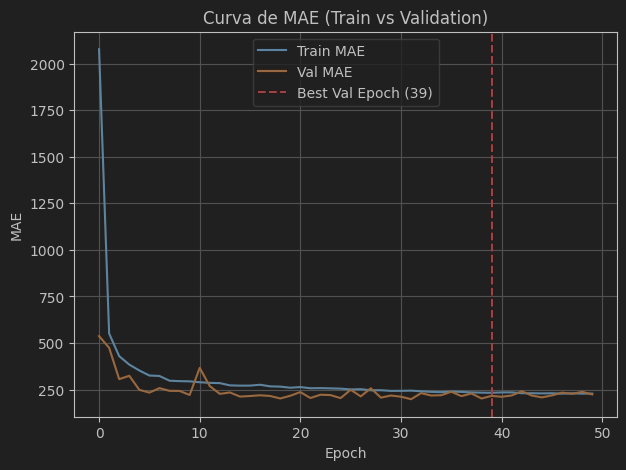
\includegraphics[width=\linewidth]{includes/cap5/graphs/sid5_mlp_mae.png}
		\subcaption{MAE}
		\vspace{0.2cm}
		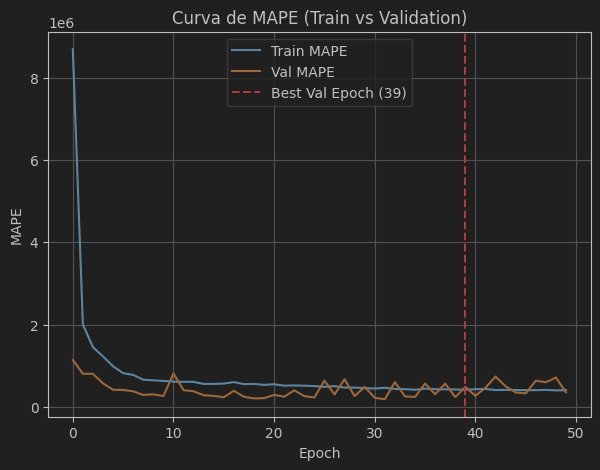
\includegraphics[width=\linewidth]{includes/cap5/graphs/sid5_mlp_mape.png}
		\subcaption{MAPE}
	\end{minipage}
	\hfill
	\begin{minipage}{0.48\textwidth}
		\centering
		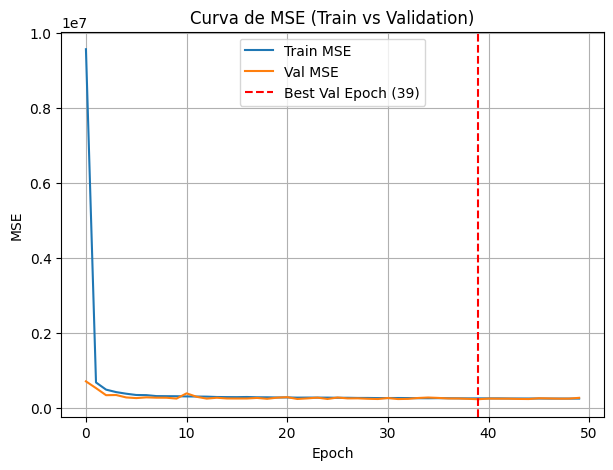
\includegraphics[width=\linewidth]{includes/cap5/graphs/sid5_mlp_mse.png}
		\subcaption{MSE}
		\vspace{0.2cm}
		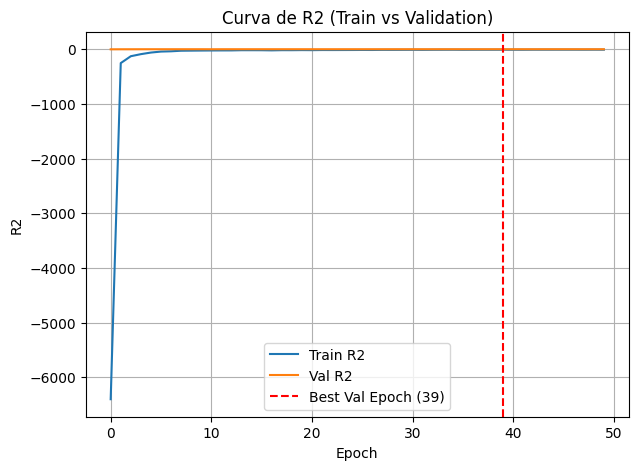
\includegraphics[width=\linewidth]{includes/cap5/graphs/sid5_mlp_r2.png}
		\subcaption{$R^2$}
		\vspace{0.2cm}
		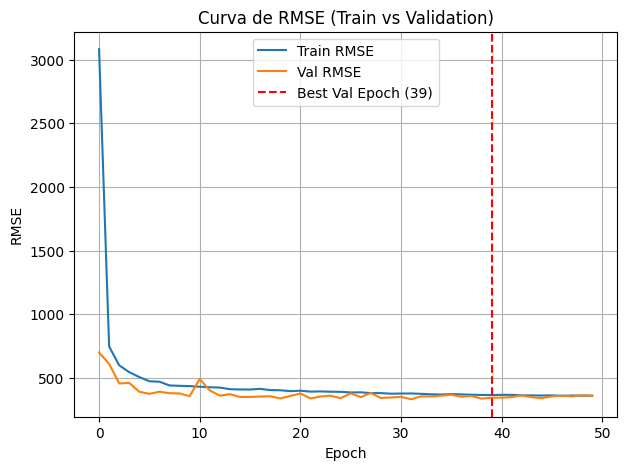
\includegraphics[width=\linewidth]{includes/cap5/graphs/sid5_mlp_rmse.png}
		\subcaption{RMSE}
	\end{minipage}
	\caption{Curvas de entrenamiento para el modelo \texttt{MLP} con sourceId 5.}
	\label{fig:curvas_sid5_mlp}
\end{figure}

\begin{figure}[H]
	\centering
	\begin{minipage}{0.48\textwidth}
		\centering
		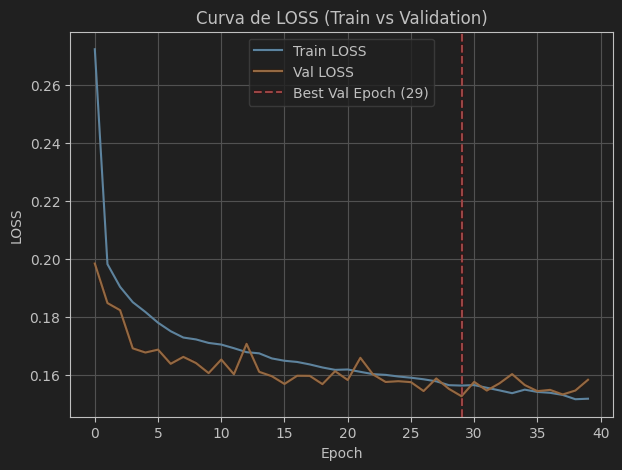
\includegraphics[width=\linewidth]{includes/cap5/graphs/sid5_trafficformer_loss.png}
		\subcaption{Loss}
		\vspace{0.2cm}
		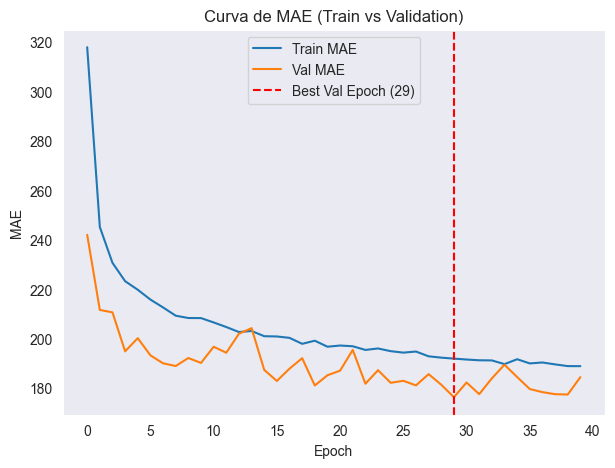
\includegraphics[width=\linewidth]{includes/cap5/graphs/sid5_trafficformer_mae.png}
		\subcaption{MAE}
		\vspace{0.2cm}
		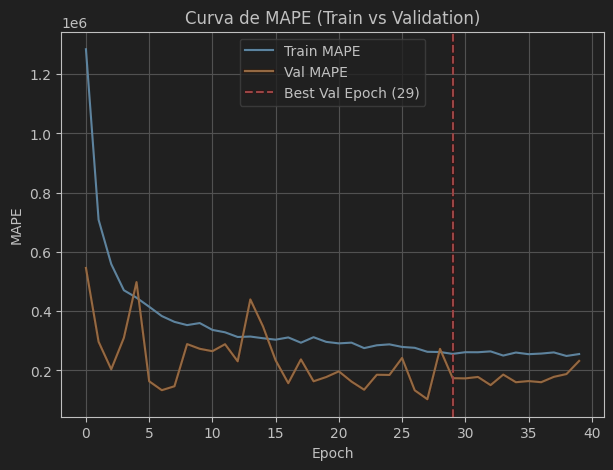
\includegraphics[width=\linewidth]{includes/cap5/graphs/sid5_trafficformer_mape.png}
		\subcaption{MAPE}
	\end{minipage}
	\hfill
	\begin{minipage}{0.48\textwidth}
		\centering
		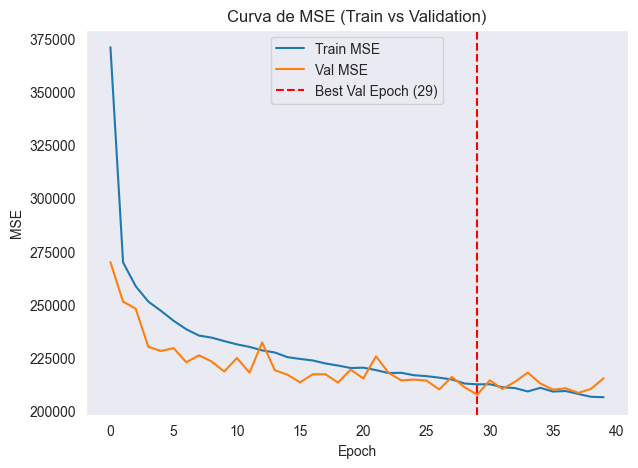
\includegraphics[width=\linewidth]{includes/cap5/graphs/sid5_trafficformer_mse.png}
		\subcaption{MSE}
		\vspace{0.2cm}
		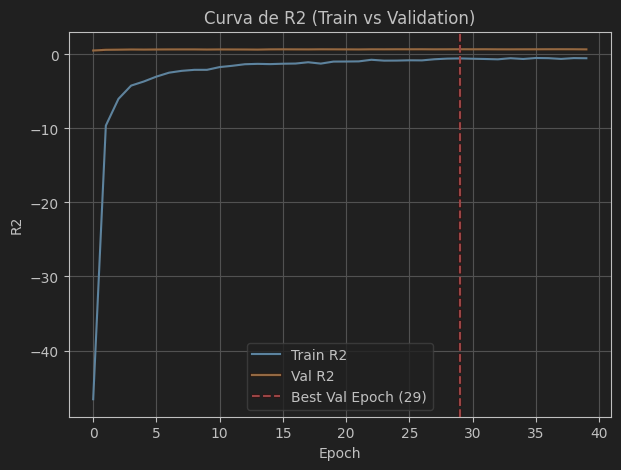
\includegraphics[width=\linewidth]{includes/cap5/graphs/sid5_trafficformer_r2.png}
		\subcaption{$R^2$}
		\vspace{0.2cm}
		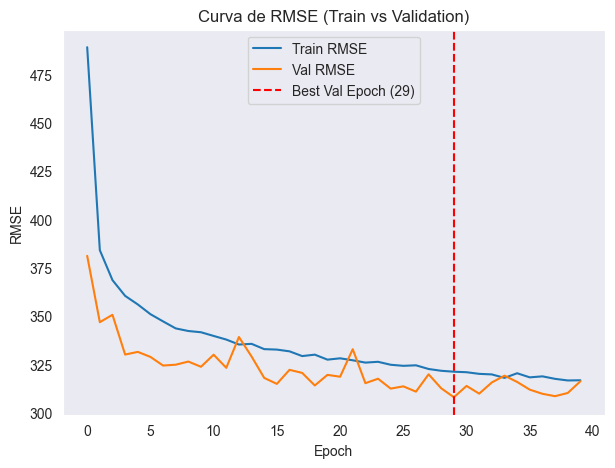
\includegraphics[width=\linewidth]{includes/cap5/graphs/sid5_trafficformer_rmse.png}
		\subcaption{RMSE}
	\end{minipage}
	\caption{Curvas de entrenamiento para el modelo \texttt{Trafficformer} con sourceId 5.}
	\label{fig:curvas_sid5_trafficformer}
\end{figure}

Todas las curvas y métricas detalladas para los 120 experimentos están disponibles en la plataforma \textit{Weights \& Biases}.

%%

\subsection{Discusión y análisis crítico}
\label{sec:discusion_analisis}

\begin{comment}
	- Interpretación de los resultados:
	- ¿Dónde y por qué Trafficformer supera a MLP?
	- ¿Hay algún caso donde no sea así?
	- Relación con lo observado en el estado del arte.
	- Reflexión sobre la influencia de los hiperparámetros, la ventana temporal y el tamaño del batch.
\end{comment}

En esta sección se realiza una evaluación crítica y comparativa de los resultados obtenidos por las dos arquitecturas propuestas (MLP y Trafficformer), para cada una de las tres fuentes de datos analizadas (sourceIds 1, 2 y 5). Se emplean las métricas reportadas en la tabla~\ref{tab:mejores_modelos}, junto con las gráficas de entrenamiento para cada modelo, para ofrecer un análisis detallado sobre la superioridad y limitaciones observadas.

\subsubsection*{Comparativa en sourceId 1}

La comparativa entre modelos MLP (figura~\ref{fig:curvas_sid1_mlp}) y Trafficformer (figura~\ref{fig:curvas_sid1_trafficformer}) muestra claramente la ventaja del modelo Trafficformer. Esta arquitectura obtiene un valor significativamente menor en las métricas de pérdida (loss), MAE, RMSE y MAPE, así como un valor superior en $R^2$. En particular, Trafficformer logra reducir el MAE desde 25.466 hasta 19.125 y el RMSE desde 38.489 hasta 30.784, mostrando una mejor capacidad para capturar las complejidades espaciales y temporales de los datos de tráfico.

El análisis visual de las curvas de entrenamiento evidencia una convergencia más rápida y estable del modelo Trafficformer, alcanzando el punto óptimo en la época 30, notablemente antes que el modelo MLP (época 67). Este fenómeno puede atribuirse a su capacidad de atención espacial y aprendizaje secuencial, permitiendo explotar eficazmente las relaciones entre sensores cercanos.

\begin{figure}[H]
	\centering
	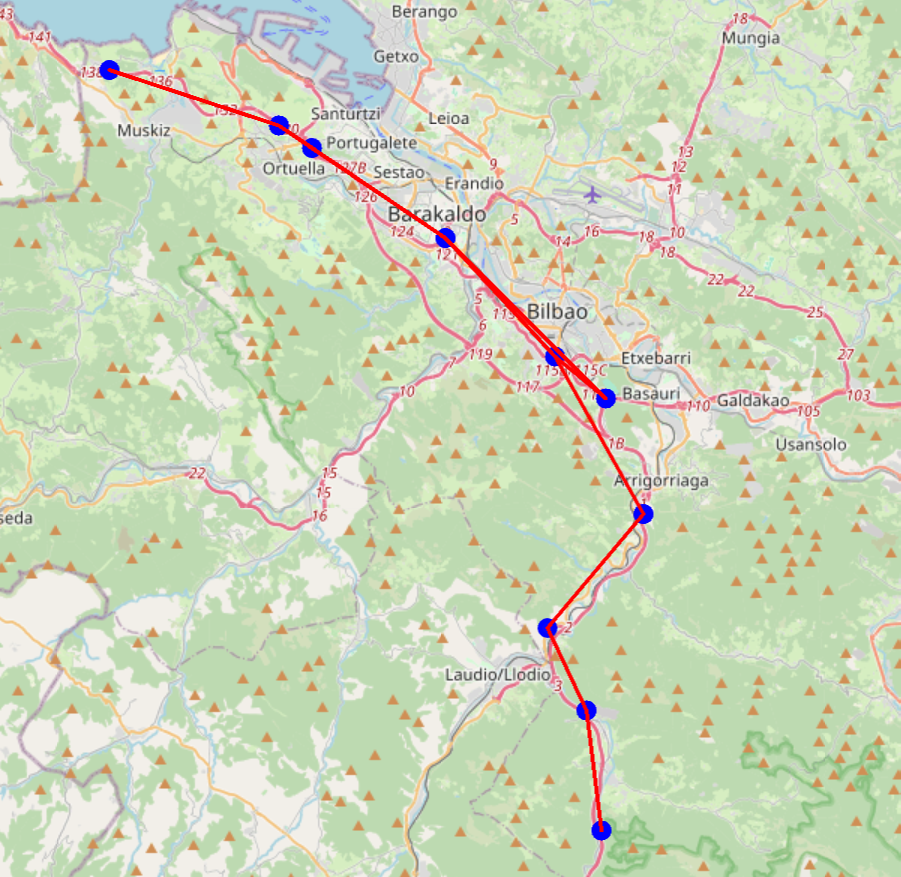
\includegraphics[width=0.7\linewidth]{includes/cap5/source_id_1_meters_mask.png}
	\caption{Distribución espacial de sensores para SourceId 1}
	\label{fig:sensores_sid1}
\end{figure}

La disposición de los sensores del SourceId 1, agrupados en puntos estratégicos específicos a lo largo de vías principales como se ve en la figura~\ref{fig:sensores_sid1}, permite al modelo Trafficformer aprovechar mejor las relaciones espaciales locales, favoreciendo su desempeño frente al modelo MLP.

\subsubsection*{Comparativa en sourceId 2}

La superioridad del modelo Trafficformer respecto al modelo MLP se acentúa aún más en los datos del sourceId 2. Como se observa en las figuras~\ref{fig:curvas_sid2_mlp} y \ref{fig:curvas_sid2_trafficformer}, Trafficformer reduce considerablemente el MAE desde 31.017 hasta 5.832 y el RMSE desde 38.177 hasta 15.046. El $R^2$ mejora sustancialmente de 0.866 (MLP) hasta 0.982 (Trafficformer), indicando una capacidad notablemente superior para explicar la variabilidad en los datos.

Las curvas de entrenamiento muestran una convergencia estable y continua del modelo Trafficformer hasta la época 96, reflejando una adecuada selección de hiperparámetros que permitió una optimización profunda. El modelo MLP, en cambio, converge rápidamente en la época 30, mostrando potencialmente limitaciones en su capacidad para aprovechar plenamente el volumen y complejidad de los datos disponibles.

\begin{figure}[H]
	\centering
	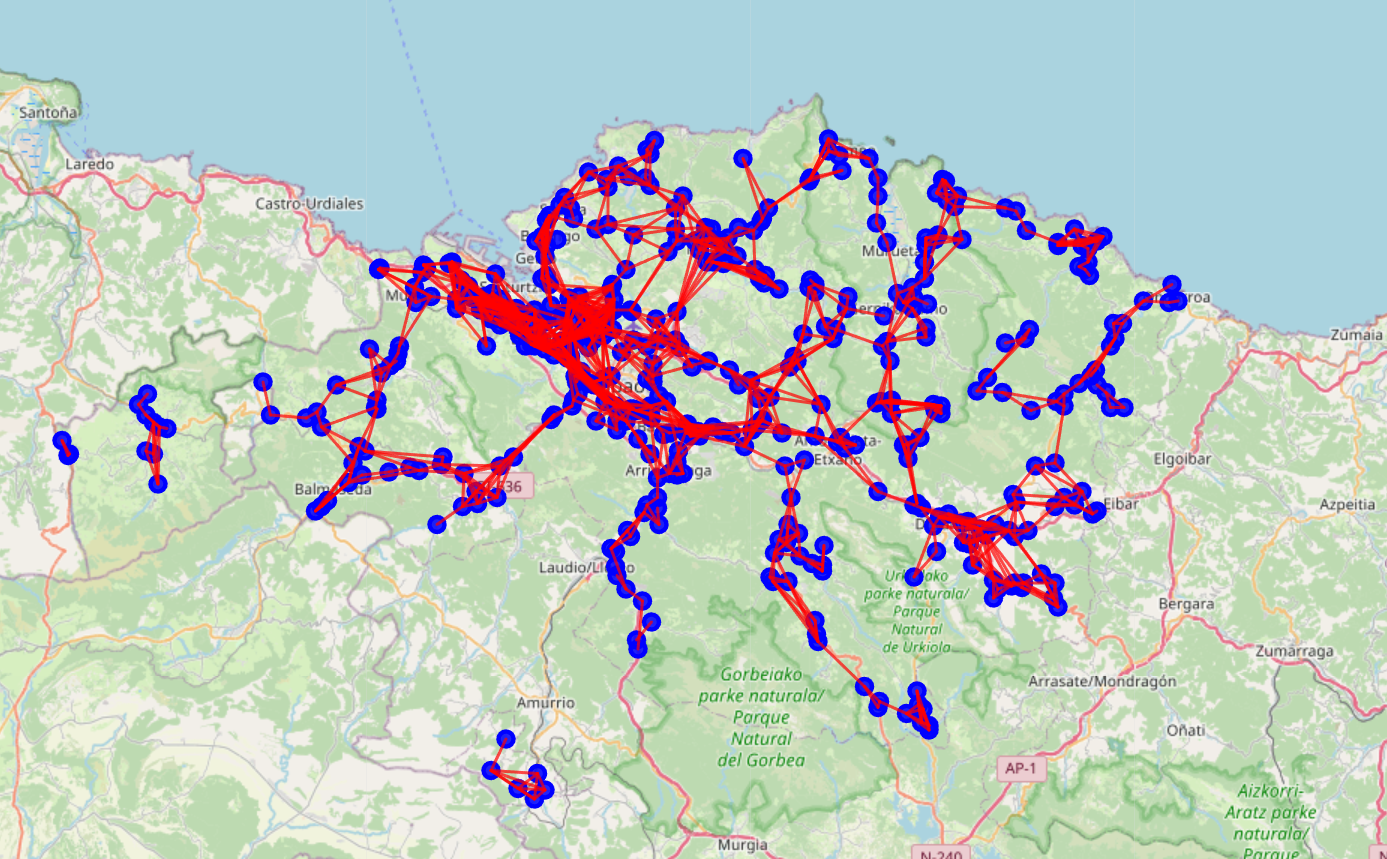
\includegraphics[width=0.7\linewidth]{includes/cap5/source_id_2_meters_mask.png}
	\caption{Distribución espacial de sensores para SourceId 2}
	\label{fig:sensores_sid2}
\end{figure}

La amplia distribución geográfica de los sensores para SourceId 2, como se aprecia en la figura~\ref{fig:sensores_sid2}, permite al modelo Trafficformer capturar relaciones espaciales complejas, aspecto que el modelo MLP no puede explotar debido a su limitada capacidad para modelar dependencias espaciales.

\subsubsection*{Comparativa en sourceId 5}

Para la fuente sourceId 5, el modelo Trafficformer sigue mostrando una clara ventaja frente al modelo MLP. Según las figuras~\ref{fig:curvas_sid5_mlp} y \ref{fig:curvas_sid5_trafficformer}, se observa una mejora en todas las métricas principales. El MAE disminuye desde 213.850 hasta 175.975, y el RMSE desde 343.603 hasta 306.134. El valor $R^2$ presenta una mejora significativa, desde un negativo e inadecuado -1.797 hasta un aceptable 0.640 para Trafficformer.

Las curvas de entrenamiento revelan que Trafficformer converge rápidamente (época 29), mostrando que el mecanismo de atención espacial resulta particularmente efectivo en escenarios urbanos densos como el representado en esta fuente de datos.

\begin{figure}[H]
	\centering
	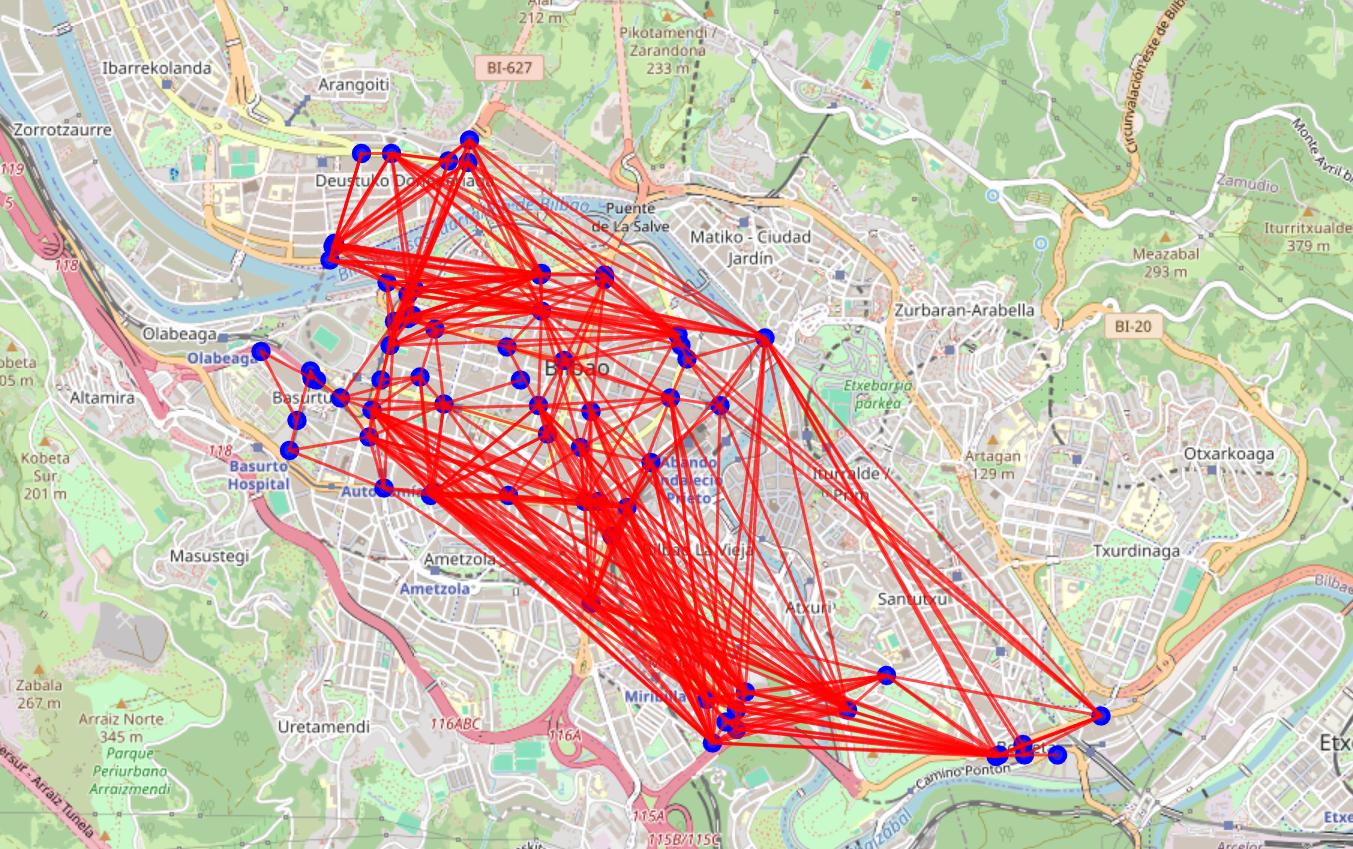
\includegraphics[width=0.7\linewidth]{includes/cap5/source_id_5_meters_mask.png}
	\caption{Distribución espacial de sensores para SourceId 5}
	\label{fig:sensores_sid5}
\end{figure}

La concentración urbana y la alta densidad espacial del SourceId 5, apreciable en la figura~\ref{fig:sensores_sid5}, generan complejas interacciones entre sensores cercanos. Esta configuración beneficia notablemente al modelo Trafficformer frente al MLP, que carece de mecanismos específicos para gestionar esta complejidad espacial.

\subsubsection*{Análisis comparativo de fuentes de datos}

Las características particulares de cada fuente de datos han ejercido una influencia importante en el desempeño de los modelos.

\paragraph{SourceId 1} Este conjunto posee un total de 386 sensores (meters), aunque estos se encuentran ubicados en unos pocos puntos estratégicos distribuidos linealmente a lo largo de vías principales, como se observa en la figura \ref{fig:sensores_sid1}. Dado que cada sensor representa un carril individual, existe una alta densidad espacial localizada en ciertas áreas críticas, pero una baja distribución geográfica. El dataset utilizado para el entrenamiento tiene una dimensionalidad de entrada de 14,828 ventanas temporales, con una longitud de secuencia (\texttt{seq\_len}) de 8 (ventanas de 4 horas). El tamaño del conjunto de entrenamiento es de 10,379, validación 2,980, y test 1,469. Esta configuración temporal amplia permite al modelo captar patrones dinámicos extendidos en el tiempo, siendo favorable para el mecanismo de atención espacial del modelo Trafficformer.

\paragraph{SourceId 2} La fuente de datos 2 presenta una distribución geográfica amplia y diversa, cubriendo exhaustivamente la red viaria de Bizkaia (figura \ref{fig:sensores_sid2}). Inicialmente se consideraron 520 sensores, aunque tras el filtrado por ausencia de datos, el número efectivo de sensores fue de 462. Esto implica una alta complejidad en términos de relaciones espaciales y diversidad de patrones de tráfico. El conjunto de entrenamiento está compuesto por 12,292 ventanas temporales, mientras que validación y test contienen 3,530 y 1,739 ventanas respectivamente. Para esta fuente se ha empleado una ventana temporal más reducida (\texttt{seq\_len} = 4, equivalentes a ventanas de 2 horas), debido a la mayor densidad y complejidad espacial. La máscara espacial generada revela numerosas conexiones entre sensores distantes, lo que beneficia significativamente al modelo Trafficformer gracias a su capacidad de capturar relaciones espaciales complejas mediante atención multi-cabezal.

\paragraph{SourceId 5} El tercer conjunto se caracteriza por una cobertura urbana densa, centrado en la ciudad de Bilbao (figura \ref{fig:sensores_sid5}). Aunque inicialmente existían 92 sensores, el filtrado redujo el número a 70. La distribución espacial en un entorno urbano tan concentrado genera relaciones espaciales complejas y altamente correlacionadas. El dataset dispone de 17,330 ventanas temporales, dividido en entrenamiento (12,131 ventanas), validación (3,483 ventanas) y test (1,716 ventanas). También se empleó una ventana de 2 horas (\texttt{seq\_len} = 4), facilitando al modelo capturar dinámicas urbanas rápidas. La máscara espacial evidencia la compleja red de interacciones espaciales entre sensores urbanos cercanos, circunstancia que nuevamente favorece al modelo Trafficformer debido a su capacidad innata para modelar dependencias espaciales y temporales simultáneamente.

Este análisis de fuentes de datos subraya la importancia del diseño experimental y la selección de ventanas temporales adecuadas a las particularidades de cada conjunto, reflejándose directamente en el rendimiento relativo de los modelos evaluados.

\subsubsection*{Síntesis y reflexión general}

La superioridad generalizada del modelo Trafficformer sobre MLP en las tres fuentes de datos analizadas se explica principalmente por la capacidad de capturar dependencias espaciales y temporales mediante el mecanismo de atención multi-cabezal. Esta capacidad es especialmente valiosa en contextos urbanos complejos (sourceId 5) y en redes de sensores extensas (sourceId 2), donde las relaciones entre los puntos de medida tienen gran relevancia.

La elección de hiperparámetros, como el tamaño del batch, learning rate, número de cabezas de atención, y dimensión de embedding, ha demostrado ser crítica en la optimización de Trafficformer. Los resultados muestran que valores intermedios o altos para \texttt{num\_heads} y \texttt{embedding\_dim} mejoran significativamente el rendimiento, validando lo observado en estudios previos del estado del arte (Chang et al., 2025).

Finalmente, el análisis pone de manifiesto que el modelo MLP presenta limitaciones inherentes a su arquitectura más simple, especialmente en contextos con fuertes correlaciones espaciales o temporales. El modelo Trafficformer, al incluir mecanismos avanzados de atención, proporciona mayor robustez y capacidad predictiva, alineándose con las tendencias recientes en la literatura científica sobre modelos Transformer aplicados a predicción del tráfico.

\subsection{Análisis avanzado de resultados por fuente de datos}
\label{sec:analisis_avanzado_resultados}

Además del análisis comparativo entre las arquitecturas y fuentes de datos realizado previamente, se ha llevado a cabo un análisis avanzado, complementario y exhaustivo, con el objetivo de identificar patrones específicos y posibles limitaciones de los modelos entrenados. Este análisis incluye gráficos específicos tales como la representación del error absoluto frente a los valores reales, series temporales comparativas para sensores individuales, mapas de errores y gráficos de distribución del error por sensor.

A continuación, se presentan las conclusiones más relevantes derivadas del análisis avanzado realizado para cada una de las fuentes de datos (\texttt{sourceId}). El detalle completo de las gráficas mencionadas está disponible en el \hyperref[anexo:analisis_avanzado]{Anexo~G}.

\paragraph{SourceId 1}
El análisis avanzado sobre la fuente de datos 1 muestra una adecuada capacidad predictiva global del modelo Trafficformer. El gráfico de dispersión (scatter plot) revela una fuerte correlación entre los valores predichos y los reales, con la mayoría de puntos cercanos a la diagonal. Sin embargo, el histograma de errores refleja la presencia de errores significativos en ciertas predicciones puntuales, lo que sugiere áreas específicas donde el modelo podría mejorar. El mapa de errores confirma visualmente que la mayoría de errores altos se concentran en puntos geográficos específicos (probablemente zonas críticas de tráfico o intersecciones complejas), lo que podría ser causado por factores no capturados completamente por el modelo.

\paragraph{SourceId 2}
En el caso del sourceId 2, se observa un excelente rendimiento del modelo Trafficformer, especialmente notable en el gráfico de dispersión y el histograma de errores, que muestran una alta concentración alrededor del valor real y errores generalmente bajos. Sin embargo, la distribución espacial del error representada en el mapa destaca algunas ubicaciones específicas con errores ligeramente mayores, posiblemente relacionadas con zonas periféricas o sensores más aislados, donde la densidad de datos disponibles para el entrenamiento fue inferior. Las series temporales para los mejores y peores sensores confirman que los mayores errores ocurren en contextos específicos, probablemente vinculados a eventos atípicos o patrones de tráfico inusuales.

\paragraph{SourceId 5}
Finalmente, la fuente de datos 5, que cubre una zona urbana densa (Bilbao), presenta una complejidad intrínseca mayor. Esto se evidencia en el gráfico de dispersión, donde se observa una mayor dispersión de los puntos respecto a la diagonal ideal, indicando predicciones menos precisas para determinados sensores urbanos. El histograma del error muestra una distribución más amplia, sugiriendo heterogeneidad en la capacidad predictiva del modelo según zonas específicas. La distribución espacial de los errores confirma que áreas urbanas densamente pobladas y congestionadas muestran consistentemente errores más elevados, un aspecto esperado dada la complejidad del tráfico urbano.

Este análisis avanzado permite concluir que, aunque el modelo Trafficformer muestra en general buenos resultados en todas las fuentes de datos, existe un margen significativo de mejora en escenarios específicos y complejos, tales como intersecciones críticas y áreas urbanas densas. Además, pone de manifiesto la importancia del análisis visual detallado para identificar oportunidades específicas de optimización en futuras iteraciones del modelo.

Las gráficas completas utilizadas para este análisis avanzado se encuentran detalladamente en el \hyperref[anexo:analisis_avanzado]{Anexo~G}.


\subsection{Limitaciones y validez de los experimentos}
\label{sec:limitaciones_validez}

\begin{comment}
	- Discusión sobre limitaciones técnicas, posibles sesgos, restricciones de hardware, tamaño de muestra, etc.
\end{comment}

Aunque los resultados obtenidos a lo largo de este trabajo demuestran una alta eficacia en la predicción del tráfico mediante las arquitecturas propuestas, es fundamental reconocer ciertas limitaciones inherentes a la investigación realizada, que deben considerarse al interpretar los resultados obtenidos y planificar futuras líneas de trabajo.

En primer lugar, existe una \textbf{limitación asociada al tamaño y representatividad de las muestras}. Aunque se han empleado datasets significativos con numerosos sensores distribuidos espacialmente, ciertas fuentes de datos (como el caso del \texttt{sourceId 1}) presentan una distribución espacial concentrada en pocos puntos estratégicos. Esto podría implicar una representación parcial del comportamiento general del tráfico en áreas menos monitorizadas o rutas secundarias.

En segundo lugar, los experimentos se han visto afectados por ciertas \textbf{restricciones técnicas y de hardware}. La necesidad de entrenar múltiples modelos complejos como Trafficformer, con elevados requerimientos computacionales, ha limitado la exploración exhaustiva del espacio de hiperparámetros, especialmente en lo relativo al número de capas, cabezas de atención o tamaño de embedding. Esta limitación técnica puede haber impedido obtener resultados aún más óptimos.

Otra limitación importante reside en la \textbf{posible presencia de sesgos en los datos originales}. Los datasets provienen de fuentes públicas (Gobierno Vasco, Diputación Foral de Bizkaia y Ayuntamiento de Bilbao), por lo que es posible que contengan sesgos derivados de errores instrumentales, pérdida de datos en algunos sensores o inconsistencias temporales en la recopilación de información. Estos sesgos pueden afectar la precisión y generalización de los modelos desarrollados.

Adicionalmente, el uso exclusivo de \textbf{variables numéricas y categóricas predefinidas} limita la capacidad del modelo para captar factores externos relevantes, como eventos específicos no registrados, cambios estacionales detallados o efectos socioeconómicos más amplios, que podrían mejorar la precisión y robustez del modelo.

Por último, la \textbf{validez externa y generalización} de los resultados está condicionada al contexto específico de la provincia de Bizkaia. Aunque la metodología aplicada es escalable y transferible a otros contextos urbanos, es necesario realizar experimentos adicionales para confirmar que los modelos desarrollados mantienen su rendimiento en otras regiones con diferentes características geográficas, culturales y económicas.

Estas limitaciones deben ser tomadas como puntos de partida para futuras investigaciones, enfocadas hacia la mejora de los modelos y la inclusión de nuevas fuentes de datos y técnicas que puedan aumentar la robustez y generalización del sistema propuesto.


